\documentclass[11pt, twoside, a4paper, openright]{report}         % This sets up the documentclass with font size and paper size already set
\usepackage[utf8]{inputenc}                                     % This will make the document use UTF-8 characters
\usepackage[danish]{babel}                                      % Changing the language to English, if this is not the default
\usepackage[T1]{fontenc}                                        % The font encoding



%%%%%%%%% GRAPHICS %%%%%%%%%%

\usepackage{graphics,graphicx}
\usepackage{epstopdf}
\usepackage{listings}                                           % OPTIONAL - This will allow for code listings in the report
\usepackage{tabularx}                                           % Allows for tables in the report
\usepackage{array, booktabs}                                    % Better table formatting
\usepackage{color}                                              % Allows for use of colours
\usepackage{xcolor}                                             % More colours

\usepackage{caption}                                            % Allows for custom cations
\captionsetup{font=footnotesize, labelfont=bf}                  % Sets the font size in the custom captions, as well as font type to bold

\usepackage{framed}                                             % Allow frames around listings and theorems

%%%%%%%% OPTIONAL LISTING MODIFIERS %%%%%%%%%

%%%%%%%% CODE %%%%%%%%%%%

% Adds code snippet functionality
\usepackage{listings}
\renewcommand{\lstlistingname}{Kodeuddrag}
\usepackage{tcolorbox}

\definecolor{commentGreen}{RGB}{34,139,24}
\definecolor{stringPurple}{RGB}{208,76,239}
\definecolor{keywordPurple}{RGB}{168,26,143}
\definecolor{indentifierPurple}{RGB}{91,44,151}
\definecolor{stringRed}{RGB}{194,29,32}
\definecolor{commentGreen}{RGB}{22,150,25}
\usepackage{tgheros}

\lstset{language=[Sharp]C,
  caption={Uddrag af C\# program},
  label=DescriptiveLabel,
  numbers=left, numberstyle=\tiny,
  backgroundcolor=\color{black!1},
}

\lstset{language=Python,
  caption={Python kode udsnit},
  label=DescriptiveLabel,
  numbers=left, numberstyle=\tiny,
  xleftmargin=\parindent,
  backgroundcolor=\color{black!1},
  basicstyle=\footnotesize\ttfamily,
  keywordstyle=\bfseries\color{keywordPurple},
  commentstyle=\itshape\color{stringRed},
  identifierstyle=\color{indentifierPurple},
  stringstyle=\color{commentGreen},
}

\lstdefinestyle{customcsharp}{
  belowcaptionskip=1\baselineskip,
  breaklines=true,
  frame=tlrb,
  rulecolor=\color{black!20},
  xleftmargin=\parindent,
  language=[Sharp]C,
  showstringspaces=false,
  basicstyle=\footnotesize\ttfamily,
  keywordstyle=\bfseries\color{keywordPurple},
  commentstyle=\itshape\color{stringRed},
  identifierstyle=\color{indentifierPurple},
  stringstyle=\color{commentGreen},
}

\lstdefinestyle{custonpython}{
  belowcaptionskip=1\baselineskip,
  breaklines=true,
  frame=tlrb,
  rulecolor=\color{black!20},
  xleftmargin=\parindent,
  language=Python,
  showstringspaces=false,
  basicstyle=\footnotesize\ttfamily,
  keywordstyle=\bfseries\color{keywordPurple},
  commentstyle=\itshape\color{commentGreen},
  identifierstyle=\color{indentifierPurple},
  stringstyle=\color{stringRed},
}

\lstdefinestyle{customasm}{
  belowcaptionskip=1\baselineskip,
  frame=L,
  xleftmargin=\parindent,
  language=[x86masm]Assembler,
  basicstyle=\footnotesize\ttfamily,
}

\lstset{escapechar=``,style=customcsharp}
\definecolor{hisyntxcolor}{rgb}{0.95, 0.95, 0.96}
\newtcbox{\hisyntx}{nobeforeafter, colback=hisyntxcolor!80,boxrule=0pt,boxsep=0pt,left=4pt,right=4pt,top=3.5pt,bottom=3.5pt,tcbox raise base}

%%%%%%%% MATHEMATICS %%%%%%%%

\usepackage{amsmath}                                            % Allign correctly
\usepackage{amssymb}                                            % More mathematica symbols
\usepackage{amsthm}                                             % Theorems
\usepackage{mdframed}
\usepackage[amssymb]{SIunits}                                   % Support SI units
\usepackage{units}                                              % Typeset units correct
\usepackage{amsfonts}                                           % Math fonts   
\usepackage{mathtools}      
\usepackage{xparse}  
%\usepackage[framed,amsmath,thmmarks]{ntheorem}                  % Allows theorems. With amsmath you can also you \eqref{label} to reference an equation

\newtheoremstyle{note}% <name>
{3pt}% <Space above>
{3pt}% <Space below>
{}% <Body font>
{}% <Indent amount>
{\itshape\bfseries\large}% <Theorem head font>
{.\newline}% <Punctuation after theorem head>
{.5em}% <Space after theorem headi>
{}% <Theorem head spec (can be left empty, meaning `normal')>
\theoremstyle{note}
\newtheorem{frtheo}{Sætning}
\newtheorem{frdef}{Definition}
\newtheorem{frlem}{Lemma}
\newtheorem{frex}{Eksempel}
\surroundwithmdframed[backgroundcolor=blue!10,linecolor=blue!10]{frtheo}
\surroundwithmdframed[backgroundcolor=blue!10,linecolor=blue!10]{frdef}
\surroundwithmdframed[backgroundcolor=blue!10,linecolor=blue!10]{frlem}
\surroundwithmdframed[backgroundcolor=blue!10,linecolor=blue!10]{frex}
\usepackage{tikz,tkz-graph,tkz-berge}
\renewcommand*{\VertexLineWidth}{1pt}%vertex thickness
\renewcommand*{\EdgeLineWidth}{1pt}% edge thickness

%%%%%%% LAYOUT %%%%%%%%

\usepackage[inner=28mm,outer=41mm,]{geometry}                   % Corrects the margins
\usepackage{titlesec}                                           % Prettier titles
\titleformat{\chapter}[hang]{                                   % Format the chapter title
    \normalfont\Huge\bfseries                                   % Format the chapter title
}{    \chaptertitlename\ \thechapter}{20pt}{\Huge}              % Format the chapter title
\titleformat*{\section}{\normalfont\Large\bfseries}             % Format section titles
\titleformat*{\subsection}{\normalfont\large\bfseries}          % Format subsection titles
\titleformat*{\subsubsection}{\normalfont\normalsize\bfseries}  % Format subsubsection titles

\usepackage{csquotes}
\usepackage{fancyhdr}                                           % Fancy headers
\pagestyle{fancy}                                               % Set the pagestyle to being fancy. This will write the chapter and page number to the header
\setlength{\headheight}{13.6pt}
\fancyhf{}                                                      % Clear the header and footer
\fancyhead[RE]{\small\nouppercase\leftmark}                     % Even pages have the chapter title
\fancyhead[LO]{\small\nouppercase\rightmark}                    % Odd pages have the section title
\fancyhead[LE,RO]{\thepage}                                     % Pagenumber on every page
\raggedbottom                                                   % Do not streach content. Instead replace it with a whitespace

\renewcommand{\headrulewidth}{0pt}                              % OPTIONAL Remove the header line seperating header and page

\usepackage{calc}                                               % Better layout formatting. Allows for arithmetics with length and such

%%%%%%% BIBLIOGRAPHY %%%%%%%%%

\usepackage[                                                    % Format of bibliography
    backend=bibtex,                                             % Use bibtex as backend manager
    style=nature,                                               % Style the bibliography right (See https://www.overleaf.com/learn/latex/Biblatex_citation_styles for more styles)
    bibencoding=utf8                                            % Encode bibliography with UTF-8 charset
]{biblatex}                                                     % Format of bibliography                           
%\bibliography{bib/mybib}

%%%%%%% GOOD TO HAVES %%%%%%%%%

\usepackage[nottoc]{tocbibind}                                  % Add bibliography to table of contents
\usepackage{lastpage}                                           % Allows you to reference the last page of the paper
\usepackage[                                                    % Adds todo notes to the document
    textwidth=\marginparwidth,                                  % Sets the text width og the todo notes as the width of the margin
    textsize=scriptsize                                         % Sets the fint size to a smaller size for more compact notes
]{todonotes}                                                    % Adds todo notes to the document

%%%%%%% REFERENCING AND LINKS %%%%%%%%

\usepackage{nameref}                                            % Allows you to refer to sections by name
\usepackage{hyperref}                                           % Enable hyperlinks and other referencing methods
\usepackage[danish]{cleveref}                                           % Better figure, table and section referencing
%\crefname{appendix}{bilag}{bilag}
%\crefname{subappendix}{bilag}{bilag}
%\crefname{subsubappendix}{bilag}{bilag}
%\crefname{section}{afsnit}{afsnit}
%\crefname{subsection}{afsnit}{afsnit}
%\crefname{subsubsection}{afsnit}{afsnit}
%\crefname{chapter}{kapitel}{kapitel}
\crefname{figure}{Figur}{Figur}
\crefname{table}{Tabel}{Tabel}
\crefname{equation}{Ligning}{Ligning}
\crefname{tikzpicture}{Graf}{Graf}
\usepackage{nameref}                                            % Load again to fix compatibility issues

\hypersetup{                                                    % Set up the pdf with correct data
	plainpages=false,                                           
	pdfauthor={Author(s)},                                      % Here you put your names
	pdftitle={Title},                                           % This should by default save it with the correct title
	pdfsubject={Subject},                                       % The subject of the report
	bookmarksnumbered=true,
	colorlinks=false,                                           % Are links coloured?
	citecolor=black,                                            % Colour of the citations
	filecolor=black,                                            % Colour of files
	linkcolor=black,                                            % Colour of links
	urlcolor=black,                                             % Colour of URLs
	pdfstartview=FitH                                           % How should the PDF scale when loaded into viewer
}

\DeclarePairedDelimiterX{\set}[1]{\{}{\}}{\setargs{#1}}
\NewDocumentCommand{\setargs}{>{\SplitArgument{1}{;}}m}
{\setargsaux#1}
\NewDocumentCommand{\setargsaux}{mm}
{\IfNoValueTF{#2}{#1} {#1\nonscript\:\delimsize\vert\allowbreak\nonscript\:\mathopen{}#2}}%
\def\Set{\set*}%
\begin{document}
\chapter{Bits}
    \section{Signed og unsigned tal}
%  |
Når en unsigned værdi konverteres til en signed værdi, er most significant bit, den bit der bestemmer om tallet er negativt eller positivt.
Denne bit har værdien $-8$, når den er signed, og derved subtraheres der for alle yderligere bits.
\begin{table}[h]
    \centering
    \begin{tabular}{c|c|c|c}
        Bits&Unsigned&Signed&Hex\\\hline
        0000&0&0&0x0\\
        0001&1&1&0x1\\
        0010&2&2&0x2\\
        0011&3&2&0x3\\
        0100&4&4&0x4\\
        0101&5&5&0x5\\
        0110&6&6&0x6\\
        0111&7&7&0x7\\
        1000&8&-8&0x8\\
        1001&9&-7&0x9\\
        1010&10&-6&0xA\\
        1011&11&-5&0xB\\
        1100&12&-4&0xC\\
        1101&13&-3&0xD\\
        1110&14&-2&0xE\\
        1111&15&-1&0xF\\
    \end{tabular}
    \caption{Tabel over signed og unsigned værdier}
\end{table}
\begin{figure}[h!]
    \centering
    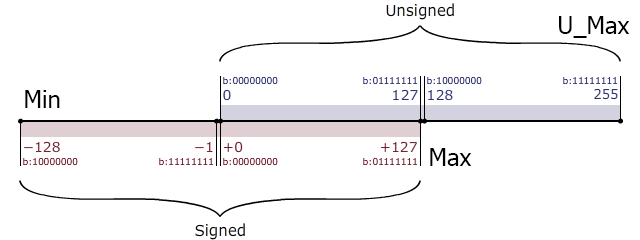
\includegraphics[width=\textwidth]{figures/signed.png}
    \caption{Signed og Unsigned komparativt}
    \label{fig:signed}
\end{figure}

    \section{Operationer}
For bits findes der operationer, som vist i DTG.
Disse er bitvise, og noteres som vist i \cref{tab:operations}.
\begin{table}[h]
    \centering
    \resizebox{\textwidth}{!}{%
    \begin{tabular}{l|l|l}
        Operation&Navn&resultat\\\hline
        x|y&eller&$1011$ Da disse bit findes i enten eller af strengene.\\
        x\&y&og&$0001$ Da denne bit deles af de to strenge.\\
        x\^y&XOR&$1010$ Da disse bits enten er i den ene eller den anden streng.\\
        ~x&negation&$1100$ Da alle bits vendes.\\
        y>>3 &Logisk højreskift&$0001$ Da bitværdien skifter 3 pladser mod højre.\\
        x<<3 &Logisk venstreskift&$1000$ Da bitværdien skifter 3 pladser mod venstre.\\
        y>>2 &Aritmetisk højreskift&$1110$ Da bitværdien skifter 3 pladser mod højre.\\
        x<<2 &Aritmetisk venstreskift&$1111$ Da bitværdien skifter 3 pladser mod venstre.\\
    \end{tabular}
    }
    \caption{Bitvise operationer og deres resultater. Der er taget udgangspunkt i $x=0011,\:y=1001$}
    \label{tab:operations}
\end{table}
For Aritmetiske skift, indsættes 1 på den nye plads, hvor ved Logiske skift, indsættes 0.
\chapter{Assembly}
Assembly sproget er det tætteste vi kommer på maskinkode.
Derfor er det essentielt for computer arkitektur faget, at undervise i dette.
    \section{x64 Assembly}
\subsection{Registre}
x64 Assembly kode har 16 64-bit registre at gøre godt med. 
Disse 16 registre kan ydermere opdeles i 32- 16- og 8-bit registre, som vist i \cref{tab:registers}
\begin{table}[h!]
    \centering
    \begin{tabular}{c|ccc|c}
        8-byte register&Bytes 0-3&Bytes 0-1&Byte 0&reg type\\\hline
        \verb|%rax|&\verb|%eax|&\verb|%ax|&\verb|%al|&Return value\\
        \verb|%rcx|&\verb|%ecx|&\verb|%cx|&\verb|%cl|&Callee value\\
        \verb|%rdx|&\verb|%edx|&\verb|%dx|&\verb|%dl|&4 argument\\
        \verb|%rbx|&\verb|%ebx|&\verb|%bx|&\verb|%bl|&3 argument\\
        \verb|%rsi|&\verb|%esi|&\verb|%si|&\verb|%sil|&2 argument\\
        \verb|%rdi|&\verb|%edi|&\verb|%di|&\verb|%dil|&1 argument\\
        \verb|%rsp|&\verb|%esp|&\verb|%sp|&\verb|%spl|&Callee saved\\
        \verb|%rbp|&\verb|%ebp|&\verb|%bp|&\verb|%bpl|&Stack pointer\\
        \verb|%r8|&\verb|%r8d|&\verb|%r8w|&\verb|%r8b|&5 argument\\
        \verb|%r9|&\verb|%r9d|&\verb|%r9w|&\verb|%r9b|&6 argument\\
        \verb|%r10|&\verb|%r10d|&\verb|%r10w|&\verb|%r10b|&Caller saved\\
        \verb|%r11|&\verb|%r11d|&\verb|%r11w|&\verb|%r11b|&Caller saved\\
        \verb|%r12|&\verb|%r12d|&\verb|%r12w|&\verb|%r12b|&Callee saved\\
        \verb|%r13|&\verb|%r13d|&\verb|%r13w|&\verb|%r13b|&Callee saved\\
        \verb|%r14|&\verb|%r14d|&\verb|%r14w|&\verb|%r14b|&Callee saved\\
        \verb|%r15|&\verb|%r15d|&\verb|%r15w|&\verb|%r15b|&Callee saved
    \end{tabular}
    \caption{Oversigt over registre i x64 Assembly}
    \label{tab:registers}
\end{table}

\subsection{Ord og bytes}
Indenfor Assembly arbejdes der med ord og bytes.
\begin{itemize}
    \item En \textit{byte} er 8 bits ($10011011$).
    \item Et \textit{word} er 2 bytes ($10011011\:10010110$).
    \item Et \textit{dword} er 4 bytes og står for double word.
    \item Et \textit{qword} er 8 bytes og står for quad word.
    \item Et \textit{oword} er 16 bytes og står for octoword.
\end{itemize}
Bogstaverne \textit{d} og \textit{q} indgår også til tider i operationer, som eksempelvis \textit{movq}.
Dette betyder blot at der flyttes noget, der er 8 byte stort.
\subsection{Instruktioner}
Mange instruktioner som mov bruger suffix som \textit{w} og \textit{q} når disse bruges.
Ydermere findes der flere forskellige former for operationer.
\subsubsection{Data flytning}
\begin{table}[h!]
    \centering
    \begin{tabular}{ll|l}
        Instruktion&Source/Destination&Beskrivelse\\\hline
        \verb|mov|&S, D&Flytter fra Source til Destination\\
        \verb|push|&S&Skubber til stakken\\
        \verb|pop|&D&Popper toppen af stakken til Destination\\\hline
        \verb|mob|&S, D&Flytter byte til word (Sign)\\
        \verb|push|&S&Flytter byte til word (Zero)\\\hline
        \verb|cwtl|&&Konverterer word i \verb|%ax| til dword i \verb|%eax| (Sign)\\
        \verb|cltq|&&Konverterer dword i \verb|%eax| til qword i \verb|%rax| (Sign)\\
        \verb|cqto|&&Konverterer qword i \verb|%rax| til oword i \verb|%rdx:%rax|
    \end{tabular}
    \caption{Instruktioner til at flytte data}
\end{table}
\subsubsection{Aritmetik}
\begin{table}[h!]
    \centering
    \begin{tabular}{ll|l}
        Instruktion&Source/Destination&Beskrivelse\\\hline
        \verb|inc|&D&Inkrementerer Destination med 1\\
        \verb|dec|&D&Dekrementerer Destination med 1\\
        \verb|neg|&D&Aritmetisk negation\\
        \verb|not|&D&Bitvis komplement
    \end{tabular}
    \caption{Unary operationer}
\end{table}
\begin{table}[h!]
    \centering
    \begin{tabular}{ll|l}
        \verb|leaq|&S, D&Indlæser effektiv addresse for Source til Destination\\
        \verb|add|&S, D&Adderer Source til Destination\\
        \verb|sub|&S, D&Subtraherer Source fra Destination\\
        \verb|imul|&S, D&Multiplerer Source med Destination\\
        \verb|xor|&S, D&Bitvis XOR Destination med Source\\
        \verb|or|&S, D&Bitvis OR Destination med Source\\
        \verb|and|&S, D&Bitvis AND Destination med Source
    \end{tabular}
    \caption{Binære operationer}
\end{table}
Instruktioner som \verb|leq 17(%rax, %rbx, 4), %rcx| skal forstås som \\\verb|%rcx = 17 + %rax + %rbx * 4|.
\begin{table}[h!]
    \centering
    \begin{tabular}{ll|l}
        \verb|sal/shl|&k, D&Venstreskift Destination med k bits\\
        \verb|sar|&k, D&Aritmetisk højreskift Destination med k bits\\
        \verb|shr|&k, D&Logisk højreskift Destination med k bits
    \end{tabular}
    \caption{Binære operationer}
\end{table}
\begin{table}[h!]
    \centering
    \begin{tabular}{ll|l}
        \verb|imulq|&S&Unsigned fuld multiplikation af \verb|%rax| med S. Resultatet gemmes i \verb|%rdx:%rax|\\
        \verb|mulq|&S&Signed fuld multiplikation af \verb|%rax| med S. Resultatet gemmes i \verb|%rdx:%rax|\\
        \verb|idivq|&S&\vtop{\hbox{\strut Signed dividering af \verb|%rdx:%rax| med S. Kvotient gemmes i \verb|%rax|.}\hbox{Rest gemmes i \verb|%rdx|}} \\
        \verb|divq|&S&\vtop{\hbox{\strut Unsigned dividering af \verb|%rdx:%rax| med S. Kvotient gemmes i \verb|%rax|.}\hbox{Rest gemmes i \verb|%rdx|}}
    \end{tabular}
    \caption{Specielle Aritmetiske operationer}
\end{table}
For operationen \verb|leaq 8(%rax, %rbx, 8)| gælder det, at det sidste 8, er et offset for addressen.
\begin{table}[h!]
    \centering
    \begin{tabular}{llll}
        \hline
        Type&Form&Værdi&Navn\\\hline
        Immediate&\verb|$imm|&\textit{imm}&Immediate\\
        Register&$r_{a}$&R[$r_{a}$]&Register\\
        Memory&\textit{imm}&M[\textit{imm}]&Absolute\\
        Memory&($r_a$)&M[R[$r_a$]]&Indirect\\
        Memory&\textit{imm}($r_b$)&M[$imm+r_b$]&Base+displacement\\
        Memory&($r_b,r_i$)&M[R[$r_b$]+R[$r_i$]]&Indexed\\
        Memory&\textit{imm}($r_i,r_b$)&M[\textit{imm} + R[$r_i$]+R[$r_b$]]&Indexed\\
        Memory&($,r_i,s$)&M[R[$r_i$]$\cdot s$]&Scaled Indexed\\
        Memory&\textit{imm}($,r_i,s$)&M[\textit{imm}+R[$r_s$]$\cdot s$]&Scaled Indexed\\
        Memory&($r_i,r_b,s$)&M[R[$r_i$]+R[$r_b$]$\cdot s$]&Scaled Indexed\\
        Memory&\textit{imm}($r_i,r_b,s$)&M[\textit{imm}+R[$r_i$]+R[$r_b$]$\cdot s$]&Scaled Indexed\\\hline
    \end{tabular}
    \caption{Memory operations}
\end{table}
\section{Y86 Assembly}
\subsection{Process stadier}
Processer kræver instruktioner, der kan organiseres som følgende.
\subsubsection{Fetch}
Her læses bytes for en instruktion, fra hukommelsen.
Dette gøres ved at bruge en Program Counter \textit{PC} som hukommelses addresse.
Disse kaldes \textbf{icode} \textit{(Instruktion kode)} og \textbf{ifun} \textit{(instruktions funktion)}.
En oversigt over disse funktionskoder kan ses i \cref{fig:icode}.
Generelt kan de siges at mængden af bytes der læses, skal adderes til \textit{PC}.
\paragraph{Icode}
Icode gives ved \verb|OP|, altså ved operationen, der udføres.
Rådfør ved \cref{fig:icode}.
\paragraph{Ifun}
Ifun gives ved funktionstypen der udføres. Igen kan der rådføres ved \cref{fig:icode}. 

\subsubsection{Decode}
Her indlæses de givne værdier for funktionen, i \verb|valA| og eller \verb|valB|.
Dette gøres oftest fra \verb|rA| og \verb|rB|, men i nogle tilfælde også \verb|%rsi|.
For instruktioner noteret $\verb|valA|\leftarrow\verb|R[...]|$ er værdien af \verb|R[...]| nummeret på det givne register, der opereres på. Se \cref{tab:y86reg}.

\subsubsection{Execute}
\verb|valE| er værdien, der gives efter \textit{Execute} blokken er kørt.
Her sættes konditions flagene \verb|ZF|, \verb|SF| og \verb|OF|, hvis der skal tjekkes for henholdsvis 0 værdi, negativ værdi eller overflow.
Samtidig noteres operationen som \verb|valx OP valy|.

\subsubsection{Memory}
Her læses eller skrives til computerens hukommelse.

\subsubsection{Writeback}
Her skrives der tilbage, når funktionen er kørt.

\subsubsection{PC update}
Program Counter opdateres.
Her gives værdien af \verb|valP|

\subsection{Registre}
Y86-Assembly har 16 registre til rådighed.
Disse 16 registre vises i \cref{tab:y86reg}
\begin{table}[h]
    \centering
    \begin{tabular}{|l|l||l|l|}
        \hline
        \verb|%rax|&0&\verb|%r8|&8\\
        \verb|%rcx|&1&\verb|%r9|&9\\
        \verb|%rdx|&2&\verb|%r10|&A\\
        \verb|%rbx|&3&\verb|%r11|&B\\
        \verb|%rsp|&4&\verb|%r12|&C\\
        \verb|%rbp|&5&\verb|%r13|&D\\
        \verb|%rsi|&6&\verb|%r14|&E\\
        \verb|%rdi|&7&Intet register&F\\\hline
    \end{tabular}
    \caption{Oversigt over registre i Y86 Assembly}
    \label{tab:y86reg}
\end{table}
Disse registre er næsten alle general purpose, dog med undtagelse af \verb|%rsp|.
\begin{figure}[h!]
    \centering
    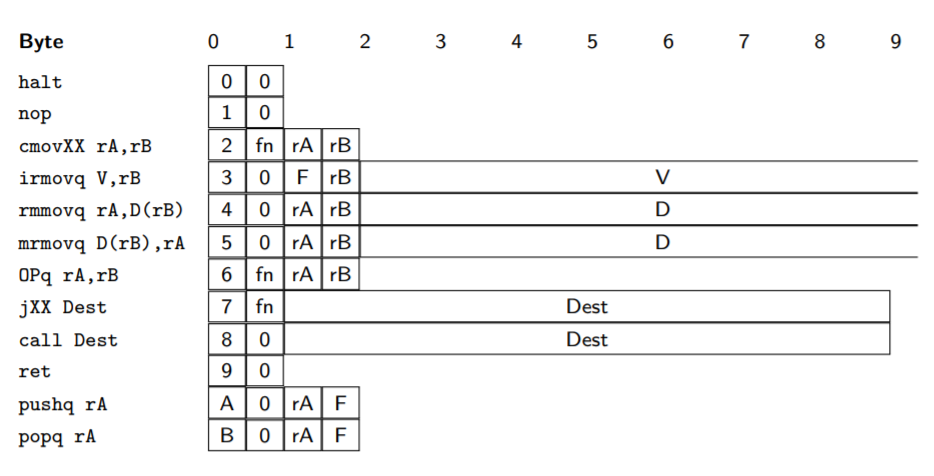
\includegraphics[width=\textwidth]{figures/icodes.png}
    \begin{tabular}{l|c|c||l}
        \hline
        \verb|rrmovq rA, rB|&2&0&Flyt fra register til register\\
        \verb|cmovle rA, rB|&2&1&Flyt hvis mindre eller lig\\
        \verb|cmovl rA, rB|&2&2&Flyt hvis mindre end\\
        \verb|cmove rA, rB|&2&3&Flyt hvis lig med\\
        \verb|cmovne rA, rB|&2&4&Flyt hvis ikke lig\\
        \verb|cmovge rA, rB|&2&5&Flyt hvis større eller lig\\
        \verb|cmovg rA, rB|&2&6&Flyt hvis større end\\\hline
        \verb|addq rA, rB|&6&0&Addition\\
        \verb|subq rA, rB|&6&1&Sutraktion\\
        \verb|andq rA, rB|&6&2&Bitvis AND\\
        \verb|xorq rA, rB|&6&3&Bitvis XOR\\\hline
        \verb|jmp Dest|&7&0&Ikke-konditionelt hop\\
        \verb|jle Dest|&7&1&Hop hvis mindre eller lig\\
        \verb|jl Dest|&7&2&Hop hvis mindre end\\
        \verb|je Dest|&7&3&Hop hvis lig med\\
        \verb|jne Dest|&7&4&Hop hvis ikke lig\\
        \verb|jge Dest|&7&5&Hop hvis større eller lig\\
        \verb|jg Dest|&7&6&Hop hvis større end\\\hline
    \end{tabular}
    \caption{Liste over instruktion- og funktionskoder}
    \label{fig:icode}
\end{figure}

\chapter{Caching}
    \section{Lokalitet}
Om lokalitet kan følgende siges.
\begin{itemize}
    \item Programmer der ofte tilgår de samme variabler har god temporal lokalitet.
    \item Programmer med \textit{Stride-k} reference mønster. 
    Jo mindre \textit{Stride} jo bedre, hvor programmer med et \textit{Stride-1} mønster, har den bedste spatialle lokalitet.
    Dette skyldes at programmet ikke skal hoppe i hukommelsen.
    \item Løkker har god temporal og spatial lokalitet, med respekt til operationerne og stride.
    Des mindre løkke-krop, des bedre lokalitet.
\end{itemize}
\chapter{Pipeline}
    En pipeline er en sekventiel udførsel af en gruppe opgaver.
Dette gør at opgavens \textit{throughput}, altså hvor hurtigt opgaven løses, stiger.
Dette kan dog også forhøje \textit{latency}, hvorved opgaven gøres langsomere.
\subsection{Throughput og Latency}
I CART måles \textit{Circuit delay} som picosekunder (ps).
I et system, hvor der eksisterer 1 blok computationel logik, med et delay på 300ps, og et register load på 20ps, gives et throughput på 3.12GIPS.
Dette kan udregnes på formlen:
\begin{equation}
    Throughput=\frac{instruktion}{delay}\cdot\frac{1000ps}{1ns}
\end{equation}
Throughput angives i GIPS \textit{(Giga-instruktioner per sekund)}, og skal derfor ganges med 1000.
Den fulde tid det tager at køre en beregning fra start til slut, kaldes latency, og er i ovenstående eksempel 320ps.
Latency i \textit{n-stage} kan udregnes ved følgende formel:
\begin{equation}
    Latency=clock\;cycler\cdot instruktion\;delay
\end{equation}
Med disse formler kan en forbedring og ny latency beregnes.
Dette gøres ved brug af følgende to formler:
\begin{equation}
    \Delta_{Throughput}= \frac{Throughput_{new}}{Throughput_{old}}
\end{equation}
\begin{equation}
    \Delta_{Latency}=\frac{Latency_{new}}{Latency_{old}}
\end{equation}
Den øgede latency skyldes at der er tilføjet mere hardware, og flere pipeline registre.
For bedre forståelse se lærebogen s. 451.
\begin{table}[h!]
    \centering
    \begin{tabular}{ll}
        \hline
        Unit&Seconds\\\hline
        1000ps&$1e^{-9}$\\
        1ns&$1e^{-9}$\\\hline
    \end{tabular}
    \caption{Convertering af Picosekunder og nanosekunder}
\end{table}
\section{Data hazard}
Data hazard forekommer, når instruktioner prøver at tilgå den samme data, under eksekvering.
Dette betyder at en instruktion, skal have skrevet tilbage, før et givent register kan bruges igen.

\chapter{Decompiling}
    Tim eksamen kan det være nyttigt at kunne decompile et program.
Dette kan gøres ved brug af kommandoen \verb|objdump -d <fil>|.
Dette producerer et dump af assembly-koden.
Denne kode er dog ikke interaktiv, og man kan derfor ikke bruge den som sådan.
Til dette kan \textit{GDB} bruges, da dette tillader interaktiv kørsel af koden under debugging.
\section{GDB debuggeren}
I stedet for at bruge standard objdump, kan GDB anvendes til at finde skjulte værdier.
Dette skyldes at GDB er en debugger for C kode, der samtidig kan skrive assembly kode, samt alle registrene.
De vigtigste kommandoer er derfor:\\
\verb|prompt> break <func_name>|\\
\verb|prompt> run|\\
\verb|prompt> nexti|\\
\verb|prompt> info reg|\\
Dette gentages indtil den givne addresse findes. 
Det kan dog være en fordel at lede efter \verb|cmp| udtryk, da disse oftests betyder at der forgår en sammenligning.
Hvis alt fejler, skal dette udregnes i hånden, med \verb|objdump|. \textit{I hope you survive}.


\chapter{Øvelser}
    \chapter{}{Kursusgang 9}
Dette afsnit vil behandle Kursusgang 9 i CART

\section{Practice Problems}
I denne sektion vil de givne Practice Problems for Kursusgangen blive gennemgået.
\section{Practice Problem 6.5}
\begin{figure}[h!]
    \centering
    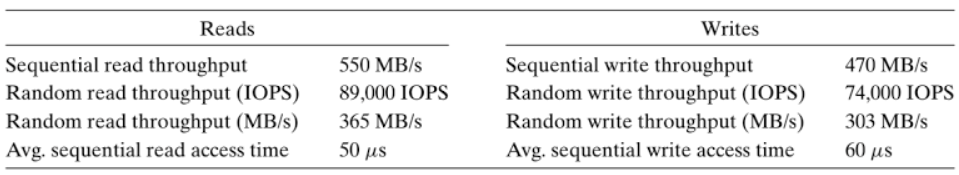
\includegraphics[width=\textwidth]{figures/ssd_props.png}
    \caption{Performance characteristics of a commercial solid state disk. 
    Source: Intel SSD 730 product specifictations. IOPS is I/O per seconds.
    throughput numbers are based on reads and writes of 4 KB blocks. (Intel SSD 730 product specifictations. Intel Cooperation)}
    \label{fig:ssd_specs}
\end{figure}
As we have seen, a potential drawback of SSDs is that the underlying flash memory can wear out.
For example, for the SSD in \cref{fig:ssd_specs}, Intel guarantees about 128 petabytes ($128\cdot 10^{15}$) of writes before the drive wears out.
Given this assumption, estimate the lifetime (in years) of this SSD for the following workloads:
\begin{enumerate}
    \item \textit{Wors case for sequential writes:} The SSD is written to continuously at a rate of 470 MB/s (The average sequential write throughput of the device).
    \item \textit{Worst case for random writes:} The SSD is written to continuously at a rate of 303 MB/s (the average random write throughput of the device)
    \item \textit{Average case:} The SSD is written to at a rate of 20 GB/day (the average daily write rate assumed by some computer manufacturers in their mobile computer workload simulations)
\end{enumerate}
\subsection{Udregninger til 6.5}
Det er givet at $1PB=10^9MB$. Samtidig vides det at der er 86400 sekunder på en dag.
\begin{enumerate}
    \item {
        Med denne information kan følgende formel bruges til at udregne levetiden for en SSD ved worst case load:
        \begin{equation}
            \left(10^9\cdot 128\right)\cdot\left(\frac{1}{470}\right)\cdot\left(\frac{1}{\left(86400\cdot 365\right)}\right) = \frac{800000}{92637} \approx 8.6359
        \end{equation}
    }
    \item {
        Samme formel kan bruges til at udregne worst case for random writes
        \begin{equation}
            \left(10^9\cdot 128\right)\cdot\left(\frac{1}{303}\right)\cdot\left(\frac{1}{\left(86400\cdot 365\right)}\right) = \frac{8000000}{597213} \approx 13.396
        \end{equation}
    }
    \item {
        Formlen kan også bruges til at udregne vores average case. 
        Dog skal sekunder ikke bruges i dette tilfælde, da der arbejdes med en tidsfaktor af dage.
        \begin{equation}
            \left(10^9\cdot 128\right)\cdot\left(\frac{1}{20000}\right)\cdot\left(\frac{1}{365}\right) = \frac{1280000}{73} \approx 17534.24658
        \end{equation}
    }
\end{enumerate}
Udregningerne er i år.
\end{document}